\section{Material und Methoden} % (fold)
    \label{sec:material_und_methoden}
    Um die Simulation durchzuführen, wurde als Modell eine Stadt mit circa 20597 Einwohnern verwendet. Die Bevölkerung unterteilt sich darin in vier sogenannte Spezies:
    \begin{enumerate}[1.]
        \item \textbf{Menschen}:
            Ganz normale Einwohner ohne besondere Fähigkeiten. Im Jäger-und-Sammler-Modell wären sie die Sammler und meiden daher den Kampf gegen Zombies.\label{species}
        \item \textbf{Helden}:
            Taffe Einwohner mit besonders ausgeprägtem Überlebensinstinkt. Sie jagen aktiv die Zombies, um sich ihr friedliches Leben zurückzuerobern.
        \item \textbf{Zombies}:
            Verseuchte Einwohner. Der Parasit hat diese ehemalig Lebenden abgetötet und steuert nun den toten Körper, um weitere Einwohner zu infizieren.
        \item \textbf{Tote}:
            Endgültig tote Einwohner, die vom Parasiten auch nicht mehr als Wirt benutzt werden können.
    \end{enumerate}
    Mit diesem Modell wurde nun ein Python-Skript entwickelt (\texttt{Methoden/simulation.py}), welches die Entwicklung der Bevölkerung, also die Anzahlen der Individuen der Spezies, über einen selbst gegebenen Zeitraum simuliert und als Plot visualisiert. Um dies möglichst realistisch und akkurat abzubilden, wurde die Simulation schrittweise erarbeitet:
    \begin{enumerate}[1.]
        \item \textbf{Normalbedingungen}\ \ 
            Zuerst wurde die Population bei gewöhnlichen Bedingungen betrachtet, also das Leben ohne Pandemie. Repräsentativ kam hier die Stadt Zülpich zur Verwendung. Diese hat Ende 2021 etwa 20597 Einwohner gehabt. In dem Jahr sind 191 lebende Kinder geboren worden, 287 Menschen gestorben, 1245 zugezogen und 991 fortgezogen \cite{zulpich}. Diese heruntergeladenen Daten sind in \texttt{Methoden/Zulpich} einsehbar und wurden für die normale Bevölkerungsentwicklung einbezogen. Dabei beeinflussen die Geburten und Todesfälle die lebende Bevölkerung, also die Menschen und Helden, prozentual, da sich bei wachsender oder sinkender Bevölkerungszahl diese allgemeinen Werte mitverändern, während die Fort- und Zuzüge mehr von der Attraktivität der Stadt abhängen, deren Einfluss hier vernachlässigt wurde.

            Umgesetzt wurde dies in der Funktion \texttt{population\_growth}. Sie verteilt die täglichen Fort- und Zuzüge gleichmäßig auf die beiden Spezies und erhöht deren Individuenzahl auch um den relativen täglichen Zuwachs/Abfall durch Geburten und Todesfällen. Dementsprechend steigt auch die Zahl der Toten.
            \label{steps:normal}
        \item \textbf{Keine Helden}\ \ 
            Die Normalbedingungen korrekt simuliert, wurde nun der Einfluss der Menschen auf die Pandemie justiert. Dementsprechend erhielten die Helden eine unveränderliche Anzahl von 0, sodass anhand von Testsimulationen aus den resultierenden Plots die \hyperref[species]{oben} beschriebene Interaktion zwischen Menschen und Zombies korrekt implementiert werden konnte.

            Die Funktion \texttt{zombie\_fights} ermittelt dabei die täglichen Begegnungen der beiden Spezies. Da jeder Zombie pro Tag einen Menschen essen will, gibt es dementsprechend so viele Kämpfe wie Zombies, oder Menschen, wenn sie in Unterzahl sind. Die Kämpfe werden dann statistisch ausgefochten, sodass ein Teil der Menschen verliert und der andere den Zombies zum Opfer fällt. Hierbei werden nun 90\% der Opfer verwandelt, während der Rest aufgefressen wird.

            Zudem gibt es noch die Funktion \texttt{human\_kills\_human}, welche einen sogenannten Chaosfaktor simulieren soll. Die Menschen sind sehr anfällig für den Stress, der durch den plötzlichen täglichen Überlebenskampf hervorgerufen wird. Das hat tödliche Auseinandersetzungen zur Folge, da Gewalt zum Alltag geworden ist. Mit einem Todesfall pro Tag soll dies umgesetzt werden, was hierbei auch Selbstmorde mit einschließt.
            \label{steps:no_heroes}
        \item \textbf{Keine Menschen}\ \ 
            Nun sollen die Helden eingebunden werden. Dazu wurde die Funktion \texttt{zombie\_fights} angepasst, sodass nun die Begegnungen mit Zombies zufällig auf die Lebenden verteilt werden, wobei die Wahrscheinlichkeiten durch den Anteil der jeweiligen Spezies zur Gesamtlebendbevölkerung bestimmt wird. Demzufolge gibt es mehr Kämpfe mit Menschen, wenn diese den Helden zahlenmäßig überlegen sind.

            Während ein Mensch mit einer Wahrscheinlichkeit von 20\% einen Kampf gewinnt, tun Helden dies aufgrund ihrer Fähigkeiten mit einer Wahrscheinlichkeit von 45\%, was sich allerdings während des ersten Monats der Pandemie auf 70\% erhöht, da sie diese Zeit benötigen, um die Schwächen der Zombies zu studieren und effiziente Strategien zu entwickeln.

            Es wurden der Funktion zwei neue Optionen hinzugefügt. Einerseits wird ein Mensch automatisch zum Held, wenn er einen Kampf mit einem Zombie überlebt, also diesen besiegt. Dies rechtfertigt sich dadurch, dass er durch das Töten unwiderruflich aus seiner Komfortzone gerissen wird. Andererseits gibt es nun auch die Möglichkeit, dass ein Mensch von einem Helden gerettet wird, der zufällig in den Kampf gerät. Das hängt auch davon ab, wie groß der Anteil an Helden ist. Wird ein Mensch gerettet, gelingt es dem Helden meist, ihn zu einem Helden zu rekrutieren. Allerdings ist jeder fünfte Gerettete nicht dazu bereit und flieht dankend.
            \label{steps:no_humans}
    \end{enumerate}
    Eine Simulation hat immer den gleichen Ablauf. Zuerst werden die Spezies mit ihrer Anzahl initialisiert. Anschließend wird für jede Iteration, also jeden simulierten Tag, zuerst \texttt{population\_growth} aufgerufen und dann die beiden Funktionen \texttt{zombie\_fights} und \texttt{human\_kills\_human} in zufälliger Reihenfolge (bei \autoref{steps:normal} natürlich ausschließlich \texttt{population\_growth}). Die Individuenzahlen nehmen während der Simulation rationale Werte an, da prozentuale Anstiege oder der tägliche Zuwachs an Geburten so am besten dargestellt werden können. Stirbt das letzte `ganze' Individuum, so wird auch der Bruchteil auf 0 gesetzt. 
    \newpage
    Um den in \autoref{steps:no_heroes} erwähnten Stressaufbau und die wachsende Gewinnwahrscheinlichkeit der Helden in \autoref{steps:no_humans} umzusetzen, wird die Sigmoid-Funktion verwendet.\par
    \begin{figure}[h]
        \centering
        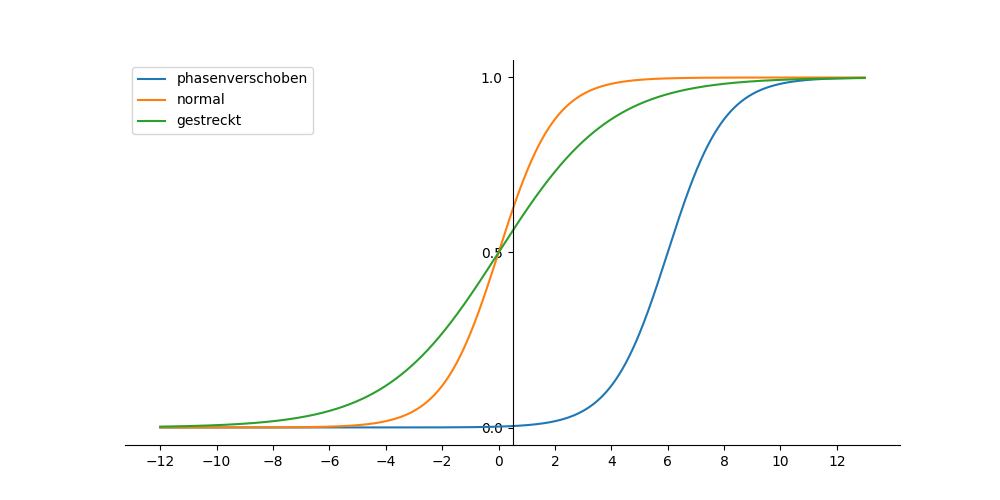
\includegraphics[width=1\textwidth]{sigmoid.png}
        \caption{Die Sigmoid-Funktion}
        \label{fig:sigmoid}
    \end{figure}
    Die Sigmoid-Funktion hat die Eigenschaft, über einen längeren Abschnitt von 0 auf 1 zu anzusteigen, was sich gut eignet, um solche nicht-lineare Entwicklungen zu simulieren. In \autoref{fig:sigmoid} sind beispielhaft drei verschiedene Varianten der Funktion dargestellt. Die normale wird über \(\frac{1}{1 + e^{-x}}\) formuliert und wechselt zwischen etwa \(-6\) und \(+6\) von 0 auf 1. Multipliziert man also \(x\) mit dem Faktor \(-\frac{6}{a}\), so wechselt die Kurve zwischen \(-a\) und \(+a\), sodass man für \(a=12\) die gestreckte Kurve in \autoref{fig:sigmoid} erhält. Subtrahiert man \(a\) von \(x\), so gelingt eine Rechts-Verschiebung entlang der x-Achse. Dies angewandt, führt dazu, dass an Tag 0 die Gewinnwahrscheinlichkeit den Wert von etwa \(0,45 + 0 \cdot 0,25 = 0,45\) annimmt und ab Tag 30 etwa \(0,45 + 1 \cdot 0,25 = 0,75\). Für den Stressfaktor gilt ähnliches Verfahren, nur dass die Funktion hier nach 100 Tagen, also bei \(x=100\) den Wert nahe 1 annimmt.
% section material_und_methoden (end)
